\documentclass[10pt, a4paper]{article}

\usepackage{appendix}
\usepackage{graphicx}
\usepackage{parskip}
\usepackage{listings}
\usepackage{caption}
\usepackage{subcaption}
\usepackage{amsmath}
\usepackage{listings}
\usepackage{xcolor}
\usepackage[most]{tcolorbox}
\usepackage{fullpage}
\usepackage{geometry}
\usepackage{tabularx}
\usepackage{gensymb}

\captionsetup{width=0.55\textwidth}

\geometry
{
    a4paper,
    total={170mm,257mm},
    left=15mm,
    top=15mm,
    right=15mm,
    bottom=20mm
}

\graphicspath{{Images/}}

%%%%%%%%%%%%%%%%%%%%%%%%%%%%%%%%%%%%%%%%%%%%%%%%%%%%%%%%%%%%%%%%%%%%%%%%%%%%%%%%%%%%%%%%%%%%%%%%%%%%%%%%%%
\begin{document}
%%%%%%%%%%%%%%%%%%%%%%%%%%%%%%%%%%%%%%%%%%%%%%%%%%%%%%%%%%%%%%%%%%%%%%%%%%%%%%%%%%%%%%%%%%%%%%%%%%%%%%%%%%
\section{Aim}
%%%%%%%%%%%%%%%%%%%%%%%%%%%%%%%%%%%%%%%%%%%%%%%%%%%%%%%%%%%%%%%%%%%%%%%%%%%%%%%%%%%%%%%%%%%%%%%%%%%%%%%%%%

The aim of the project is to design and build an autonomous rover system that could be used in a remote location without direct supervision. 

\begin{figure} [h!]
    \centering
    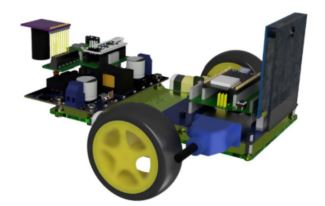
\includegraphics[scale=0.8]{Rover.JPG}
\end{figure}

The rover will have the following main functionalities:
\begin{itemize}
    \item Receive movement commands and send status data through a processing unit.
    \item Detect and avoid obstacles in its working area.
    \item Build a map of its local working area including obstacles on an offsite data store.
    \item A charging station will be designed and implemented to charge the rover batteries.
\end{itemize}

%%%%%%%%%%%%%%%%%%%%%%%%%%%%%%%%%%%%%%%%%%%%%%%%%%%%%%%%%%%%%%%%%%%%%%%%%%%%%%%%%%%%%%%%%%%%%%%%%%%%%%%%%%
\section{Timeline}

\begin{itemize}
    \item \textbf{11 - May}: Introductory session
    \item \textbf{12 - May} - \textbf{26 - May}: Design and practice sessions 
    \item \textbf{14 - June} - \textbf{25 - June}: Assessment period 
\end{itemize}

%%%%%%%%%%%%%%%%%%%%%%%%%%%%%%%%%%%%%%%%%%%%%%%%%%%%%%%%%%%%%%%%%%%%%%%%%%%%%%%%%%%%%%%%%%%%%%%%%%%%%%%%%%
\section{Deliverables}

\begin{itemize}
    \item Report containing:
    \begin{itemize}
        \item Design process of the Mars Rover 
        \item Technical specifications and details of components
        \item Reflection essay on coursework lecture 
    \end{itemize}

    Report should \textbf{not exceed} 40 pages.

    \item Video demo on Mars Rover operation 
    \item Oral exam 
\end{itemize}


%%%%%%%%%%%%%%%%%%%%%%%%%%%%%%%%%%%%%%%%%%%%%%%%%%%%%%%%%%%%%%%%%%%%%%%%%%%%%%%%%%%%%%%%%%%%%%%%%%%%%%%%%%
\section{Project submodules}

The Mars Rover project is composed of six submodules which are managed by each individual member of the team. 

\subsection{EEE: Drive (Alyson)}

Drive subsystem handles the movement of the rover, parts including the frame, motors and optical flow sensor.

Responsibilities:
\begin{itemize}
    \item Direction control
    \item Distance measurement
    \item Speed control 
    \item Turning method 
\end{itemize}

\subsection{EEE: Energy (Ivy)}

Energy subsystem handles the power system of the rover, provided through the solar panels.

Responsibilities:
\begin{itemize}
    \item Battery charge profile design 
    \item Battery charge status estimation 
    \item Battery balancing algorithms 
    \item Charge batteries 
    \item Prevent explosion/melt
    \item PV MMPT algorithm
\end{itemize}

\subsection{EEE: Integration (Izzah)}

Combines the subsystems of the rover together.

Responsibilities:
\begin{itemize}
    \item Developing the central processor of the rover and ensuring correct functionality of all sub-systems.
    \item Manage communications between the onboard rover systems and the cloud command processes.
    \item Build, maintain and assist in debugging the other modules. 
\end{itemize}

\subsection{EIE: Command (Xin)}

Allows remote control of the rover by connecting to the control subsystem and accessible via a web browser/mobile app.

Responsibilities:
\begin{itemize}
    \item  Create a web or mobile dashboard to control the rover remotely and receive information from the different subsystems. 
\end{itemize}

\subsection{EIE: Control (Igor)}

Using ESP32 microcontroller, handles communication with all the subsystems via different communication protocols. The ESP32 will have a unique IP address and will be used as an access point.

Responsibilities:
\begin{itemize}
    \item  Communication management between:
    \begin{itemize}
        \item Motors 
        \item FPGA 
        \item Cloud command 
        \item Charging station 
    \end{itemize}
\end{itemize}

\subsection{EIE: Vision (Ebby)}

Enables the rover to detect and avoid obstacles to achieve its target destination. 

Responsibilities:
\begin{itemize}
    \item  Use on-board vision and software to identify obstructions and objects of interest such as:
    \begin{itemize}
        \item Move the robot around the terrain according to instructions from cloud command.
        \item Avoiding obstructions.   
        \item Closed loop monitoring of position.   
        \item Sending commands to the motor control. 
    \end{itemize}
\end{itemize}

\pagebreak

\section{Project management}

Due to the nature of the sub-systems, module development are relatively independent. Particular care should be placed on the following sub-systems:
\begin{itemize}
    \item Command (EIE) 
    \item Control (EIE)
    \item Integration (EEE)
\end{itemize}
as it handles the end-points and data flow of the systems.

\begin{figure} [h!]
    \centering
    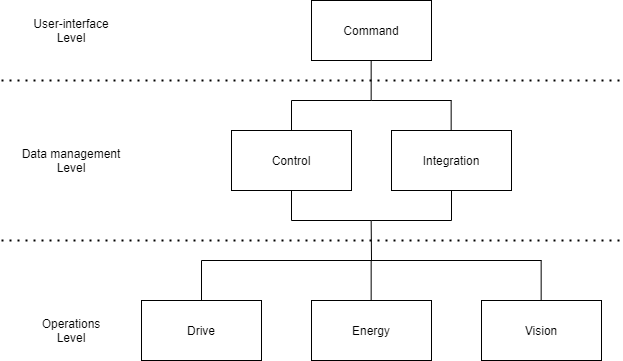
\includegraphics[scale=0.6]{project heirarchy.png}
    \caption{Project sub-system hierarchy}
\end{figure}

Project sub-system heirarchy represents the different layers in the rover system that each handles different aspects that brings the overall system together. Any changes in the base layers needs to notify the respective upper layers to ensure compatibility is met.

\begin{itemize}  
    \item \textbf{User-interface level}: Responsible for the user experience aspect of the rover system and, ensuring a stable and seamless communication link between the rover and user interface. 
    
    \item \textbf{Data management level}: Serves as the bridge between the user and the functional sub-systems. 
    
    \textit{Integration} serves as the oversight component of the Operations level, providing neccessary support and communication between all the respective modules. This module also ensures and records all testing done in each of the sub-systems.

    \item \textbf{Operations level}: Critical in ensuring correct rover operation in each of their respective domains. 
\end{itemize}

\pagebreak

\section{Project management}

Due to the nature of the sub-systems, module development are relatively independent. Particular care should be placed on the following sub-systems:
\begin{itemize}
    \item Command (EIE) 
    \item Control (EIE)
    \item Integration (EEE)
\end{itemize}
as it handles the end-points and data flow of the systems.

\begin{figure} [h!]
    \centering
    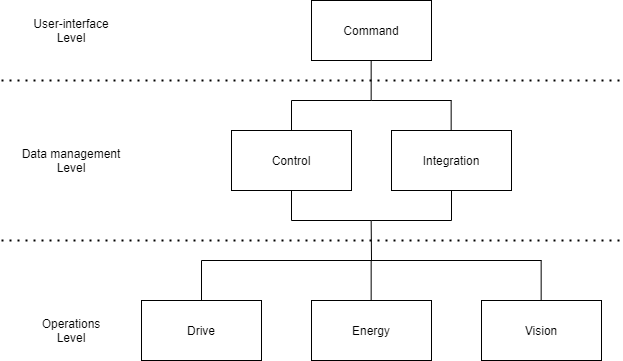
\includegraphics[scale=0.6]{project heirarchy.png}
    \caption{Project sub-system hierarchy}
\end{figure}

Project sub-system heirarchy represents the different layers in the rover system that each handles different aspects that brings the overall system together. Any changes in the base layers needs to notify the respective upper layers to ensure compatibility is met.

\begin{itemize}  
    \item \textbf{User-interface level}: Responsible for the user experience aspect of the rover system and, ensuring a stable and seamless communication link between the rover and user interface. 
    
    \item \textbf{Data management level}: Serves as the bridge between the user and the functional sub-systems. 
    
    \textit{Integration} serves as the oversight component of the Operations level, providing neccessary support and communication between all the respective modules. This module also ensures and records all testing done in each of the sub-systems.

    \item \textbf{Operations level}: Critical in ensuring correct rover operation in each of their respective domains. 
\end{itemize}

\pagebreak

\section{Assessment breakdown}

\begin{itemize}
    \item $40$\%: Design \textbf{[Report + Oral]} 
    \begin{itemize}
        \item $40$\%: Design process from problem definition to implementation
        \item $20$\%: Structural design of Rover
        \item $20$\%: Functional design for Rover and for each module
        \item $10$\%: Inter-module communication 
        \item $10$\%: Project management 
    \end{itemize}

    \item $40$\%: Implementation \textbf{[Report + Oral + Video]} 
    \begin{itemize}
        \item $50$\%: Rover operation
        \item $30$\%: Module implementation 
        \item $20$\%: Problem solving (case with evidence)
    \end{itemize}

    \item $20$\%: Personal statement \textbf{[Oral + Personal statement]} 
    \begin{itemize}
        \item $100$\%: Confidential personal statement
    \end{itemize}
\end{itemize}

\subsection{Design}

This component will dictate the overall themes and structure of the report. Main design themes of importance is:
\begin{enumerate}
    \item Energy efficiency 
    \item User to system confirmation 
    \item Minimalism to reduce failure points 
\end{enumerate}

Terms to clarify:
\begin{itemize}
    \item \textbf{Structural design}: Design based on the actual physical structure of the rover 
    \begin{itemize}
        \item Due to height of vision camera, care is taken to scan carefully 
        \item Chart for data flow between submodules
    \end{itemize}
    \item \textbf{Functional design}: Design based on the intended functionalities of the rover 
\end{itemize}

The last two points (Inter-module communication + Project management) will be handled together with the following evidence provided:
\begin{itemize}
    \item Project management chart
    \item Meeting minutes 
    \item Communication heirarchy chart 
\end{itemize}

\subsection{Implementation}

Report will mainly handle "Module implementation" and "Problem solving":
\begin{itemize}
    \item \textbf{Module implementation}:
    
    Brief summary of how each sub-module functions, use ample diagrams to simplify the explanations.

    \item \textbf{Problem solving}: 
    
    Our team spans four countries so it is a great starting perspective to talk about. Potential links to "Project Management" component.
\end{itemize}

\pagebreak

\subsection{Personal statement}

Personal statement will include:
\begin{itemize}
    \item Which other students did you help, and in what way?
    \item Who helped you, and in what way?
    \item What was your experience. For each student, or their communication: was this prompt, clear, and honest?
    \item Is there anyone on your team who you feel has particularly contributed more or less than average (give reasons)?
\end{itemize}


%%%%%%%%%%%%%%%%%%%%%%%%%%%%%%%%%%%%%%%%%%%%%%%%%%%%%%%%%%%%%%%%%%%%%%%%%%%%%%%%%%%%%%%%%%%%%%%%%%%%%%%%%%
\end{document}
%%%%%%%%%%%%%%%%%%%%%%%%%%%%%%%%%%%%%%%%%%%%%%%%%%%%%%%%%%%%%%%%%%%%%%%%%%%%%%%%%%%%%%%%%%%%%%%%%%%%%%%%%%